%!TEX TS-program = pdflatex
%!TEX root = i3det-top.tex
%!TEX encoding = UTF-8 Unicode

% (KDH) put overall electrical connection schematic diagram in 
% this section and include some brief details on cable specs 
% 19 AWG (to be confirmed) and 
 
\section{Cable Systems}

The IceCube detector may be viewed as a digital network of optical
sensors. The IceCube cable systems form the physical backbone of this
network, supplying simultaneously power to the DOMs and bi-directional
digital communications between the DOMs and the readout hardware at the
surface. Copper was chosen over optical fiber at an early stage in the
project due to concerns with mechanical robustness of fiber during
freeze-in in the deep ice and a previous successful demonstration of the
digitally-readout optical modules contained within the AMANDA detector
(String 18).

The Cable System is comprised of the following assemblies: Surface to DOM
Cable, Surface Junction Box (SJB), Surface Cable, ICL In-Ice Quad Patch
Cable and IceTop Cables. The Surface to DOM Cable, 2505m long, is deployed
into the ice along with 60 DOMs that are attached to connectors at 30
breakouts spaced 34m apart. Each pair of DOMs is connected to a unique
single twisted wire pair. Wire pairs are combined into a 4 conductor quad
cable that enables its meeting electrical performance requirements. The 60
DOMs on each cable require 15 quads. An additional 5 quads in the Surface
to DOM Cable provide for special instrumentation connections, a spare quad
and hard local coincidence connections between adjacent DOMs. The Surface
to DOM Cable terminates at the surface in the Surface Junction Box located
in the IceTop tank pit. The Surface Junction Box is a stainless steel
enclosure that houses the Surface to DOM Cable and Surface Cable
connections. IceTop Cables also terminate and connect to the Surface Cable
in the Surface Junction Box. The Surface Cable is trenched 1m deep into the
surface of the snow between the IceTop tank pit and the ICL. The Surface
Cables vary in length from 300m to approximately 800m in length and were
made to a custom length depending on hole location. The Surface Cables are
pulled into the ICL and terminate at a patch rack where the individual
quads are separated and connected to ICL In-Ice Quad Patch Cables or Icetop
Patch Cables that finally terminate at the DOMHub or IceTop DOMHub. Each
DOMHub services a single in-ice string (see
Fig.~\ref{fig:icecube-cables-logical}). 

\begin{figure}
  \centering
  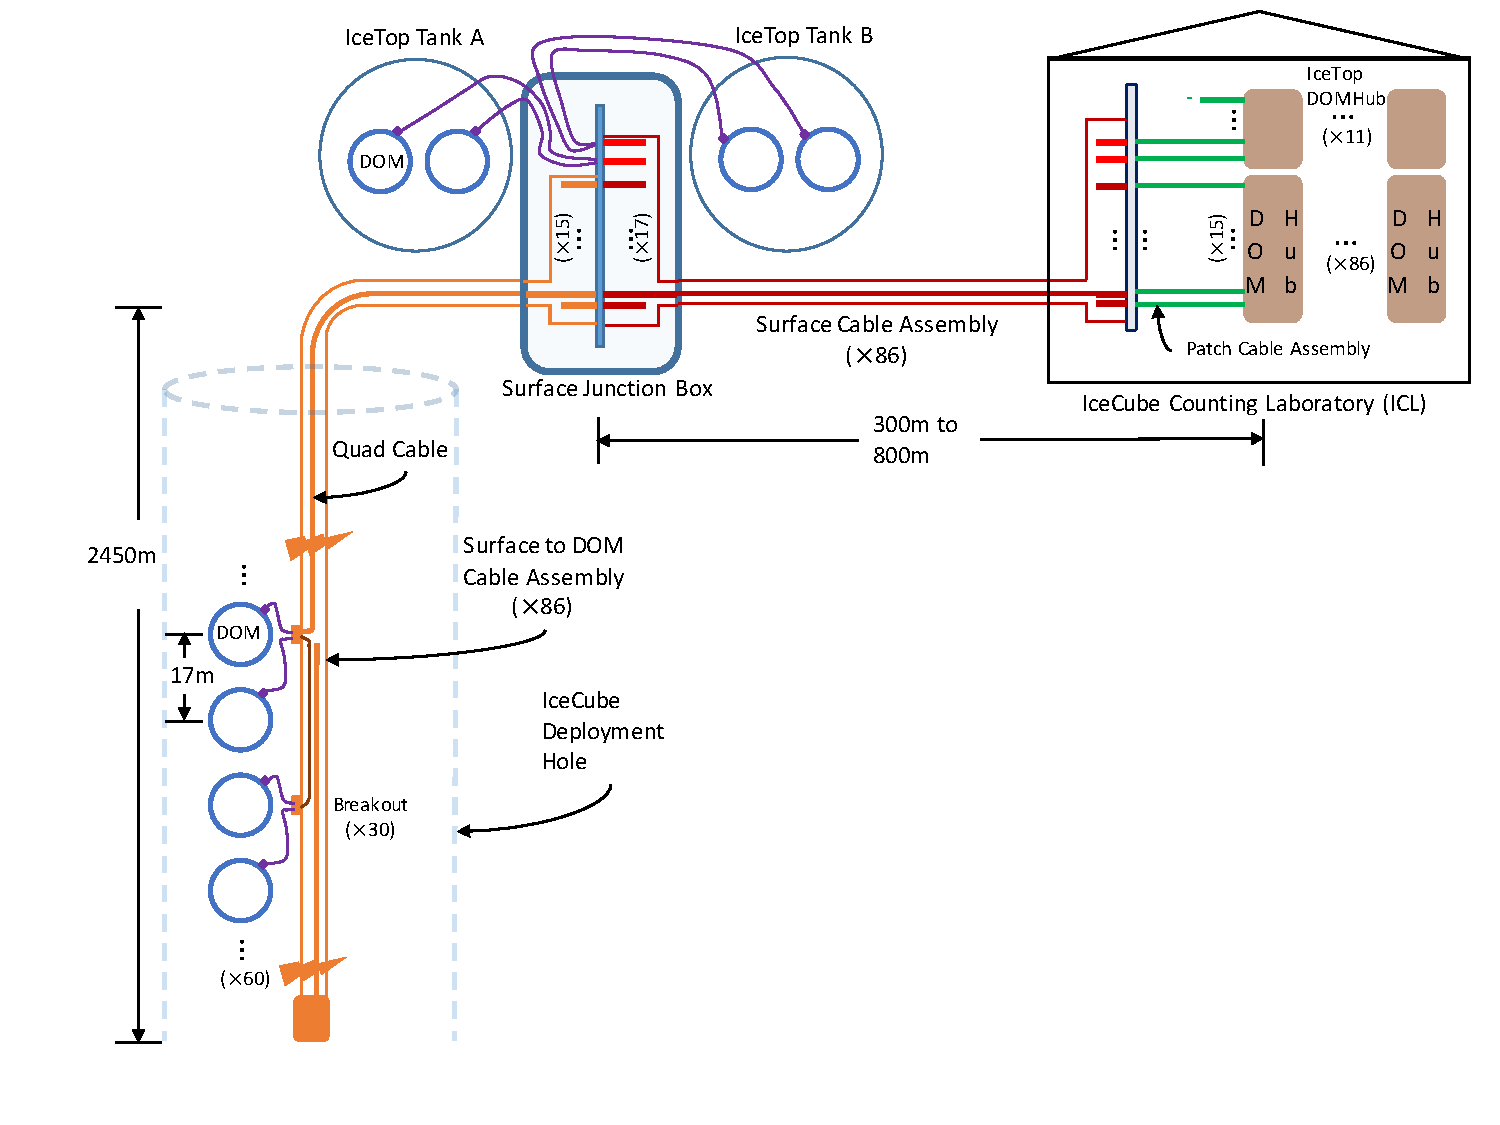
\includegraphics[width=0.95\textwidth]{graphics/cables/cable_system_schematic.pdf}
  \caption{\label{fig:icecube-cables-logical}Schematic of the IceCube cable network architecture.}
\end{figure}

The IceCube Cable System design had to meet a technically challenging
variety of mechanical, electrical and functional requirements in order for
IceCube to meet its science objectives. Most significantly, the Cable
System design had to satisfy these requirements under the extreme
conditions of installation at the South Pole. This is particularly the case
for the Surface to DOM Cable that also had to withstand hydrostatic
overpressures of up to 450 bar while deployed. All items had to survive the
rigors of transportation to the South Pole along with the capability to be
stored at temperatures down to $-70$C without performance
degradation. Handling temperatures were specified down to $-40$C for all
cable components. The main electrical requirements were applied to the quad
cable which are stated in Table ~\ref{tab:quad_requirements}.

% FIX ME CLEAN UP TABLE
\begin{table}[h]
  \centering
  \begin{tabularx}{\textwidth}{| l | X | X | }
    \hline
    \bf{Test} & \bf{Limit} & \bf{Conditions} \\
    \hline

    attenuation & 20 dB maximum & at 1.0 MHz end-to-end \\
    \hline

    crosstalk attenuation & intra-quad \& quad-quad & \\
    \hline

    & 50 dB minimum & 100 kHz to 2.0 MHz \\
    \cline {2-3}
    NEXT & 50 dB minimum at 2.0 MHz & decreasing 15 dB / decade \\
    \cline {2-3}
    & 24 dB minimum & at 100 MHz \\
    \hline

    & 30 dB minimum & 100 kHz to 2.0 MHz \\
    \cline {2-3}
    ELFEXT & 30 dB minimum at 2.0 MHz & decreasing 20 dB / decade \\
    \cline {2-3}
    & 10 dB minimum & at 20 MHz \\
    \hline

    differential impedance & $145\Omega \pm 10\Omega$ & at 1.0 MHz \\
    \hline

    loop resistance & $160\Omega$ maximum & \\
    \hline

    hipot & 2000 VDC minimum, 1.0 $\mu A$ maximum leakage, 60 second
    minimum duration & all conductors individually tested with all other
    conductors grounded \\
    \hline    
  \end{tabularx}
  \caption{Electrical requirements for the cable quads.} 
  \label{tab:quad_requirements}
\end{table}

 The Surface to DOM cable was also required to be less than 50mm in
 diameter, weigh less than 2 kg / m, have a minimum bend radius of 40cm,
 carry a maximum static tensile load of 10kN, and have a breaking strength
 of 40kN. The final Surface to DOM design can be seen in
 Fig.~\ref{fig:cable_xsection}.  

\begin{figure}
  \centering
  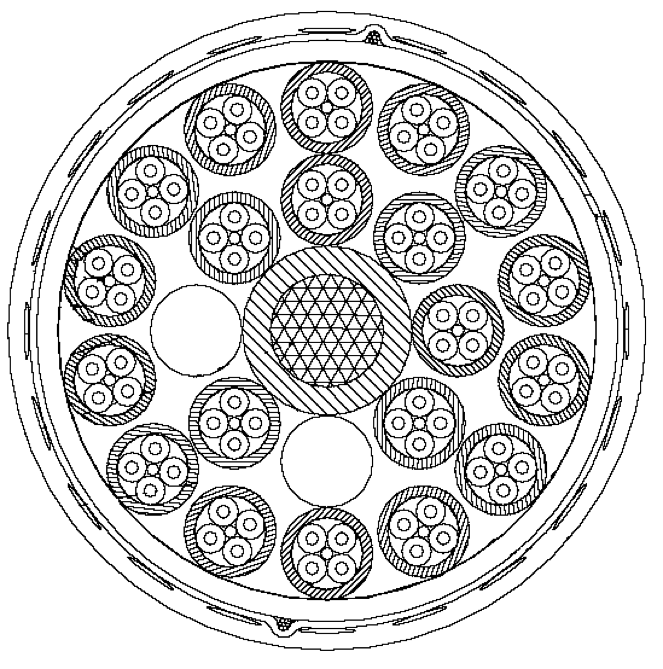
\includegraphics[width=0.5\textwidth]{graphics/cables/cable_xsection.png}
  \caption{\label{fig:cable_xsection}Surface to DOM Cable cross
    section. Nominal 46mm diameter with cable mass of 2 kg/m.} 
\end{figure}

The cable includes 20 quads, 2 polyethylene fillers to maintain structural
symmetry, Kevlar outer and inner core strength members, a copper foil
shield with drain wires to provide electrical noise isolation and water
block that prevented any water or ice from damaging the symmetry of the
cable. The final Surface Cable design has a similar construction to the
Surface to DOM Cable with the exception of the water block and Kevlar
strength members. In addition, a bundle of 3 shielded quads and a bundle of
6 shielded power wires replace the inner Kevlar strength member and service
the IceTop Station that is made up of 2 tanks, each with 2 DOMs.

A competitive proposal process resulted in 2 main suppliers for the IceCube
Cable System. Ericsson Network Technologies (Hudiksvall, Sweden) was chosen
to produce the raw cable and Seacon Brantner \& Associates Inc. (El Cajon,
California) was picked to manufacture the actual cable assemblies. The raw
cable was manufactured and tested to meet all required specifications prior
to shipment. A Certificate of Conformance was provided for each cable along
with individual test reports. The longer Surface to DOM Cables were then
wound on to custom metal spools while the shorter Surface Cables were wound
onto wooden spools. The cables were shipped via sea vessel from Sweden,
through the Panama Canal, to Long Beach, California where they were
offloaded to trucks for delivery to Seacon. Seacon provided the breakouts
and the end termination for the Surface to DOM Cable and the end
terminations for the Surface Cable. The connectors used for the Surface to
DOM to DOM interface were the Seacon glass reinforced epoxy XSJJ
connector. The 30 breakouts per Surface to DOM Cable were installed by
slicing open the cable, cutting the correct quads, terminating them to the
XSJJ connectors, waterproofing and overmolding the connectors and then
resealing the cable. The breakout manufacturing process needed to be a
reliable and repeatable method since the cable not only had to withstand
the operating environment but also the rigors of deployment. Seacon also
attached 120 Yale Cordage (Saco, Maine) Yalegrips to the Surface to DOM
Cable that served as mechanical attachment points for the 60 deployed DOMs
per cable. The separate quads in each cable were terminated with military
style (MS) round, metal shell connectors. After cable assembly is complete,
each cable was individually tested for continuity and subject to hi-pot
testing. The cables were then transported to the Port Hueneme (California)
Operations center that is the hub for United States Antarctic Program
(USAP) logistics in the U.S. The cables were loaded onto a ship each
December for delivery to McMurdo Station in January where they are stored
for the austral winter outside subject to extreme temperatures. In the
following November, they were then loaded onto LC-130 Herc cargo planes for
delivery to the South Pole.

Installation of the IceCube Cable System at the South Pole each season was
broken into 5 distinct tasks. The tasks were Surface Cable trenching and
installation into the ICL and SJB, Surface to DOM Cable deployment and
connection to the SJB, IceTop Power and Data installation at the ICL and
IceTop trench, patch cable installation in the ICL, and, testing,
troubleshooting and repair after all connections were made. Surface Cables
were installed early in the season as IceTop freeze control operations
required a connection back to the ICL. A 1m deep trench was mechanically
dug between the ICL and each IceTop station. After the cable was placed in
the trench, it was pulled into the ICL and connected to the IceTop
DOMHub. Later, just prior to filling the tanks with water in the field, the
connections were made between the Surface Cable and the SJB. The IceTop
DOMs with their long 17m penetrator assemblies were connected to the
appropriate quad located in center of the Surface Cable. Two additional
cables were connected between the SJB and the tanks that powered and
communicated with the IceTop Freeze Control Units. The Surface to DOM Cable
was prepared for installation while the enhanced hot water drill was coming
up the hole in its reaming phase. After removal of the drill head, the
Surface to DOM cable was pulled into the Drill Tower and DOM deployment
commenced. Surface to DOM Cable deployment and Surface Cable installation
were not dependent on each other. IceTop drove the Surface Cable
installation while drilling and DOM deployment operations drove the Surface
to DOM Cable installation schedule. After DOM deployment was complete, the
Surface to DOM cable was taken off the spool and dragged to the IceTop
station where its connection to the Surface Cable in the SJB was
made. Finally, patch cables were installed in the ICL between the
individual quads and the DOMHub in the ICL. End to end string commissioning
now commenced.
